% Gemini theme
% https://github.com/anishathalye/gemini
%
% We try to keep this Overleaf template in sync with the canonical source on
% GitHub, but it's recommended that you obtain the template directly from
% GitHub to ensure that you are using the latest version.

\documentclass[final]{beamer}

% ====================
% Packages
% ====================

\usepackage[T1]{fontenc}
\usepackage{lmodern}
\usepackage[size=custom,width=120,height=72,scale=1.0]{beamerposter}
\usetheme{gemini}
\usecolortheme{gemini}
\usepackage{graphicx}
\usepackage{booktabs}
\usepackage{tikz}
\usepackage{pgfplots}

% ====================
% Lengths
% ====================

% If you have N columns, choose \sepwidth and \colwidth such that
% (N+1)*\sepwidth + N*\colwidth = \paperwidth
\newlength{\sepwidth}
\newlength{\colwidth}
\setlength{\sepwidth}{0.025\paperwidth}
\setlength{\colwidth}{0.25\paperwidth}

\newcommand{\separatorcolumn}{\begin{column}{\sepwidth}\end{column}}

% ====================
% Title
% ====================

\title{Generating KSHV Deletion Mutant to Study the Effect of Viral GPCR's}

\author{Nicholas Carey \inst{1}}

\institute[shortinst]{\inst{1} UC Berkeley}

% ====================
% Body
% ====================

\begin{document}

\begin{frame}[t]
\begin{columns}[t]
\separatorcolumn

\begin{column}{\colwidth}

  \begin{block}{Introduction}
Kaposi’s Sarcoma associated herpesvirus (KSHV), also known as Human Herpes Virus 8 (HHV-8), is a cancer-causing virus responsible for Kaposi’s Sarcoma, Pulmonary Effusion Lymphoma, and multicentric Castleman’s disease.5 KSHV is sexually transmitted and often establishes a life-long infection. It is estimated that 5-20\% of the United States population is infected with KSHV. While KSHV infections are asymptomatic in most immunocompetent people, those with compromised immune systems often develop cancer. This puts people with AIDS or transplant recipients at higher risk from infection and development of malignant tumors and lesions, normally in the mouth, face, GI and Respiratory tracts.  It is estimated that infection rates among HIV positive individuals are much higher, around 20-50\% demonstrating substantial seroprevalence. In regions where HIV/AIDS epidemics are worse, such as Sub-Saharan Africa, the rate of KSHV infection is even higher.5 The focus of this experiment will be to study an open reading frame (ORF) from the KSHV genome. Our hope is that, by learning how this specific ORF affects KSHV infections, better treatments and methods of prevention for Kaposi’s Sarcoma and other KSHV/gamma-herpesvirus related diseases will be developed in the future. 
  \end{block}

  \begin{alertblock}{Methods}

    This block catches your eye, so \textbf{important stuff} should probably go
    here.

    Curabitur eu libero vehicula, cursus est fringilla, luctus est. Morbi
    consectetur mauris quam, at finibus elit auctor ac. Aliquam erat volutpat.
    Aenean at nisl ut ex ullamcorper eleifend et eu augue. Aenean quis velit
    tristique odio convallis ultrices a ac odio.

    \begin{itemize}
      \item \textbf{Fusce dapibus tellus} vel tellus semper finibus. In
        consequat, nibh sed mattis luctus, augue diam fermentum lectus.
      \item \textbf{In euismod erat metus} non ex. Vestibulum luctus augue in
        mi condimentum, at sollicitudin lorem viverra.
      \item \textbf{Suspendisse vulputate} mauris vel placerat consectetur.
        Mauris semper, purus ac hendrerit molestie, elit mi dignissim odio, in
        suscipit felis sapien vel ex.
    \end{itemize}

    Aenean tincidunt risus eros, at gravida lorem sagittis vel. Vestibulum ante
    ipsum primis in faucibus orci luctus et ultrices posuere cubilia Curae.

  \end{alertblock}

\end{column}

\separatorcolumn

\setlength{\colwidth}{0.4\paperwidth}
\begin{column}{\colwidth}

  \begin{block}{Results}
  	\begin{columns}[t, totalwidth=\textwidth]
    	\begin{column}{0.49\linewidth}
    	Some sample text to see the size of a sub-column in the Results section.
        \begin{figure}
      	  \centering
          a)
     		 \includegraphics[width=0.25\linewidth]{Photos/WT_phase.png}
          b)
             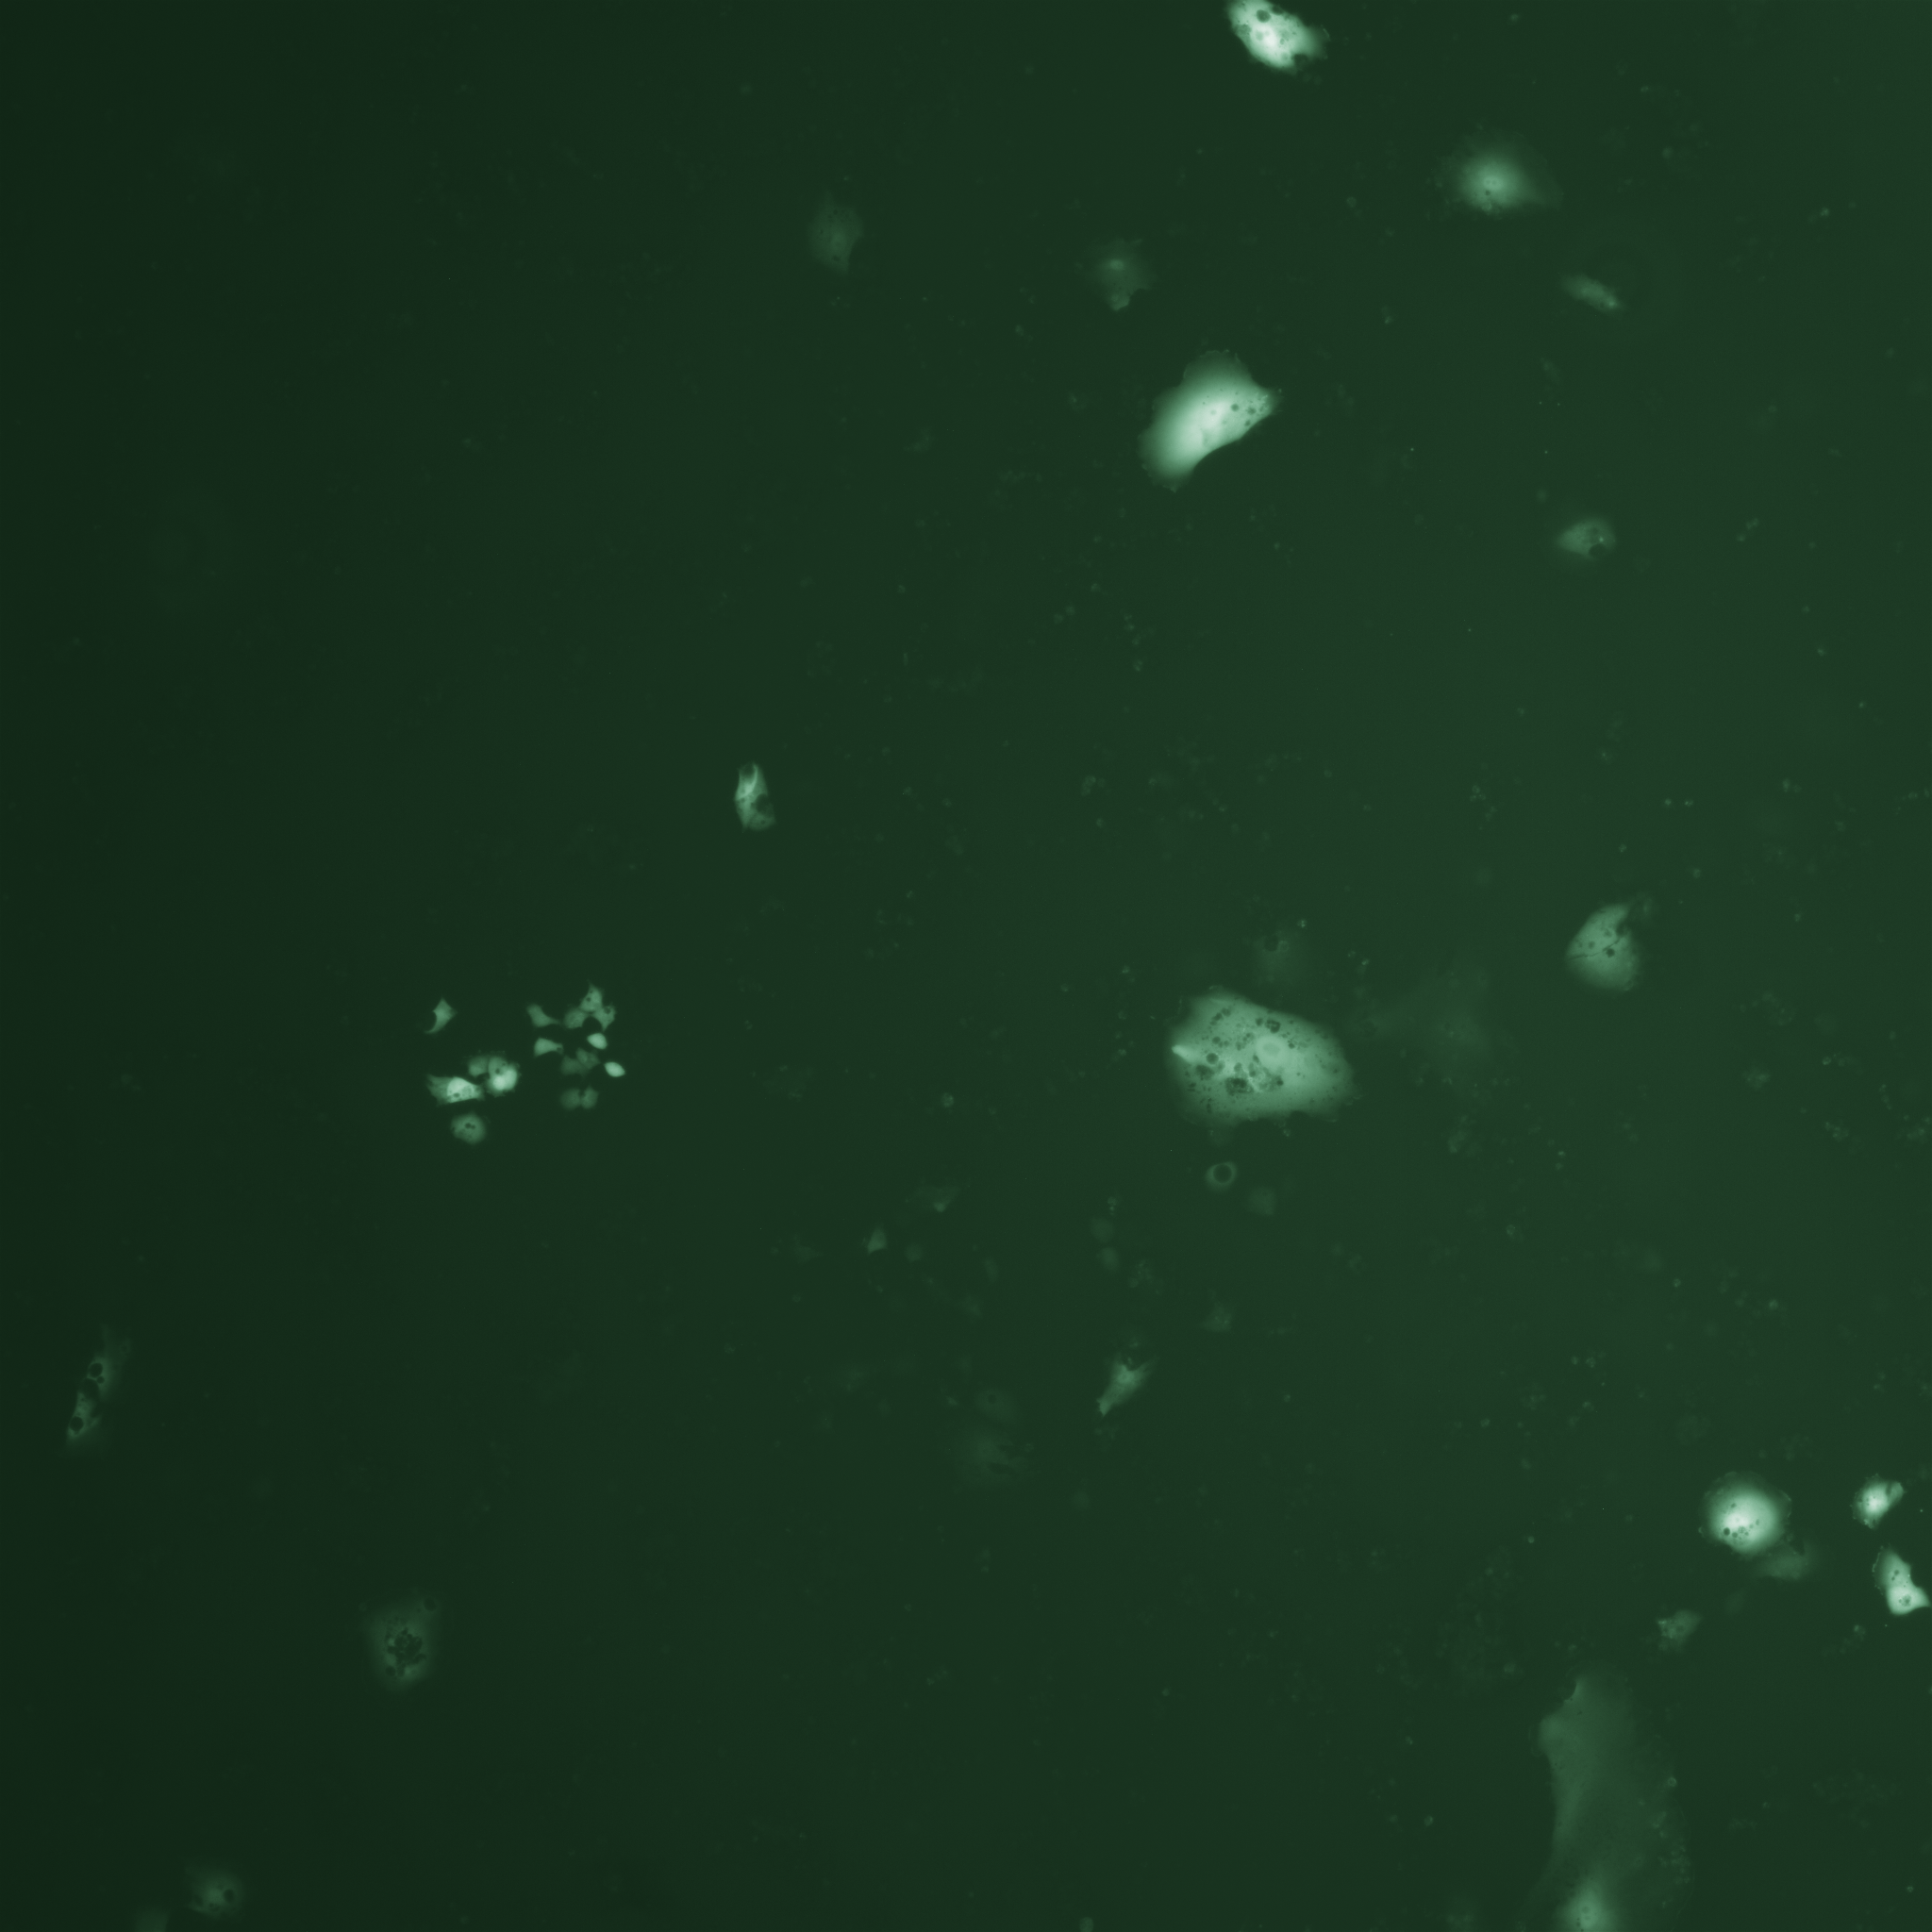
\includegraphics[width=0.25\linewidth]{Photos/WT_GFP.png}\\
          c)
             \includegraphics[width=0.25\linewidth]{Photos/74_phase.png}
          d)
             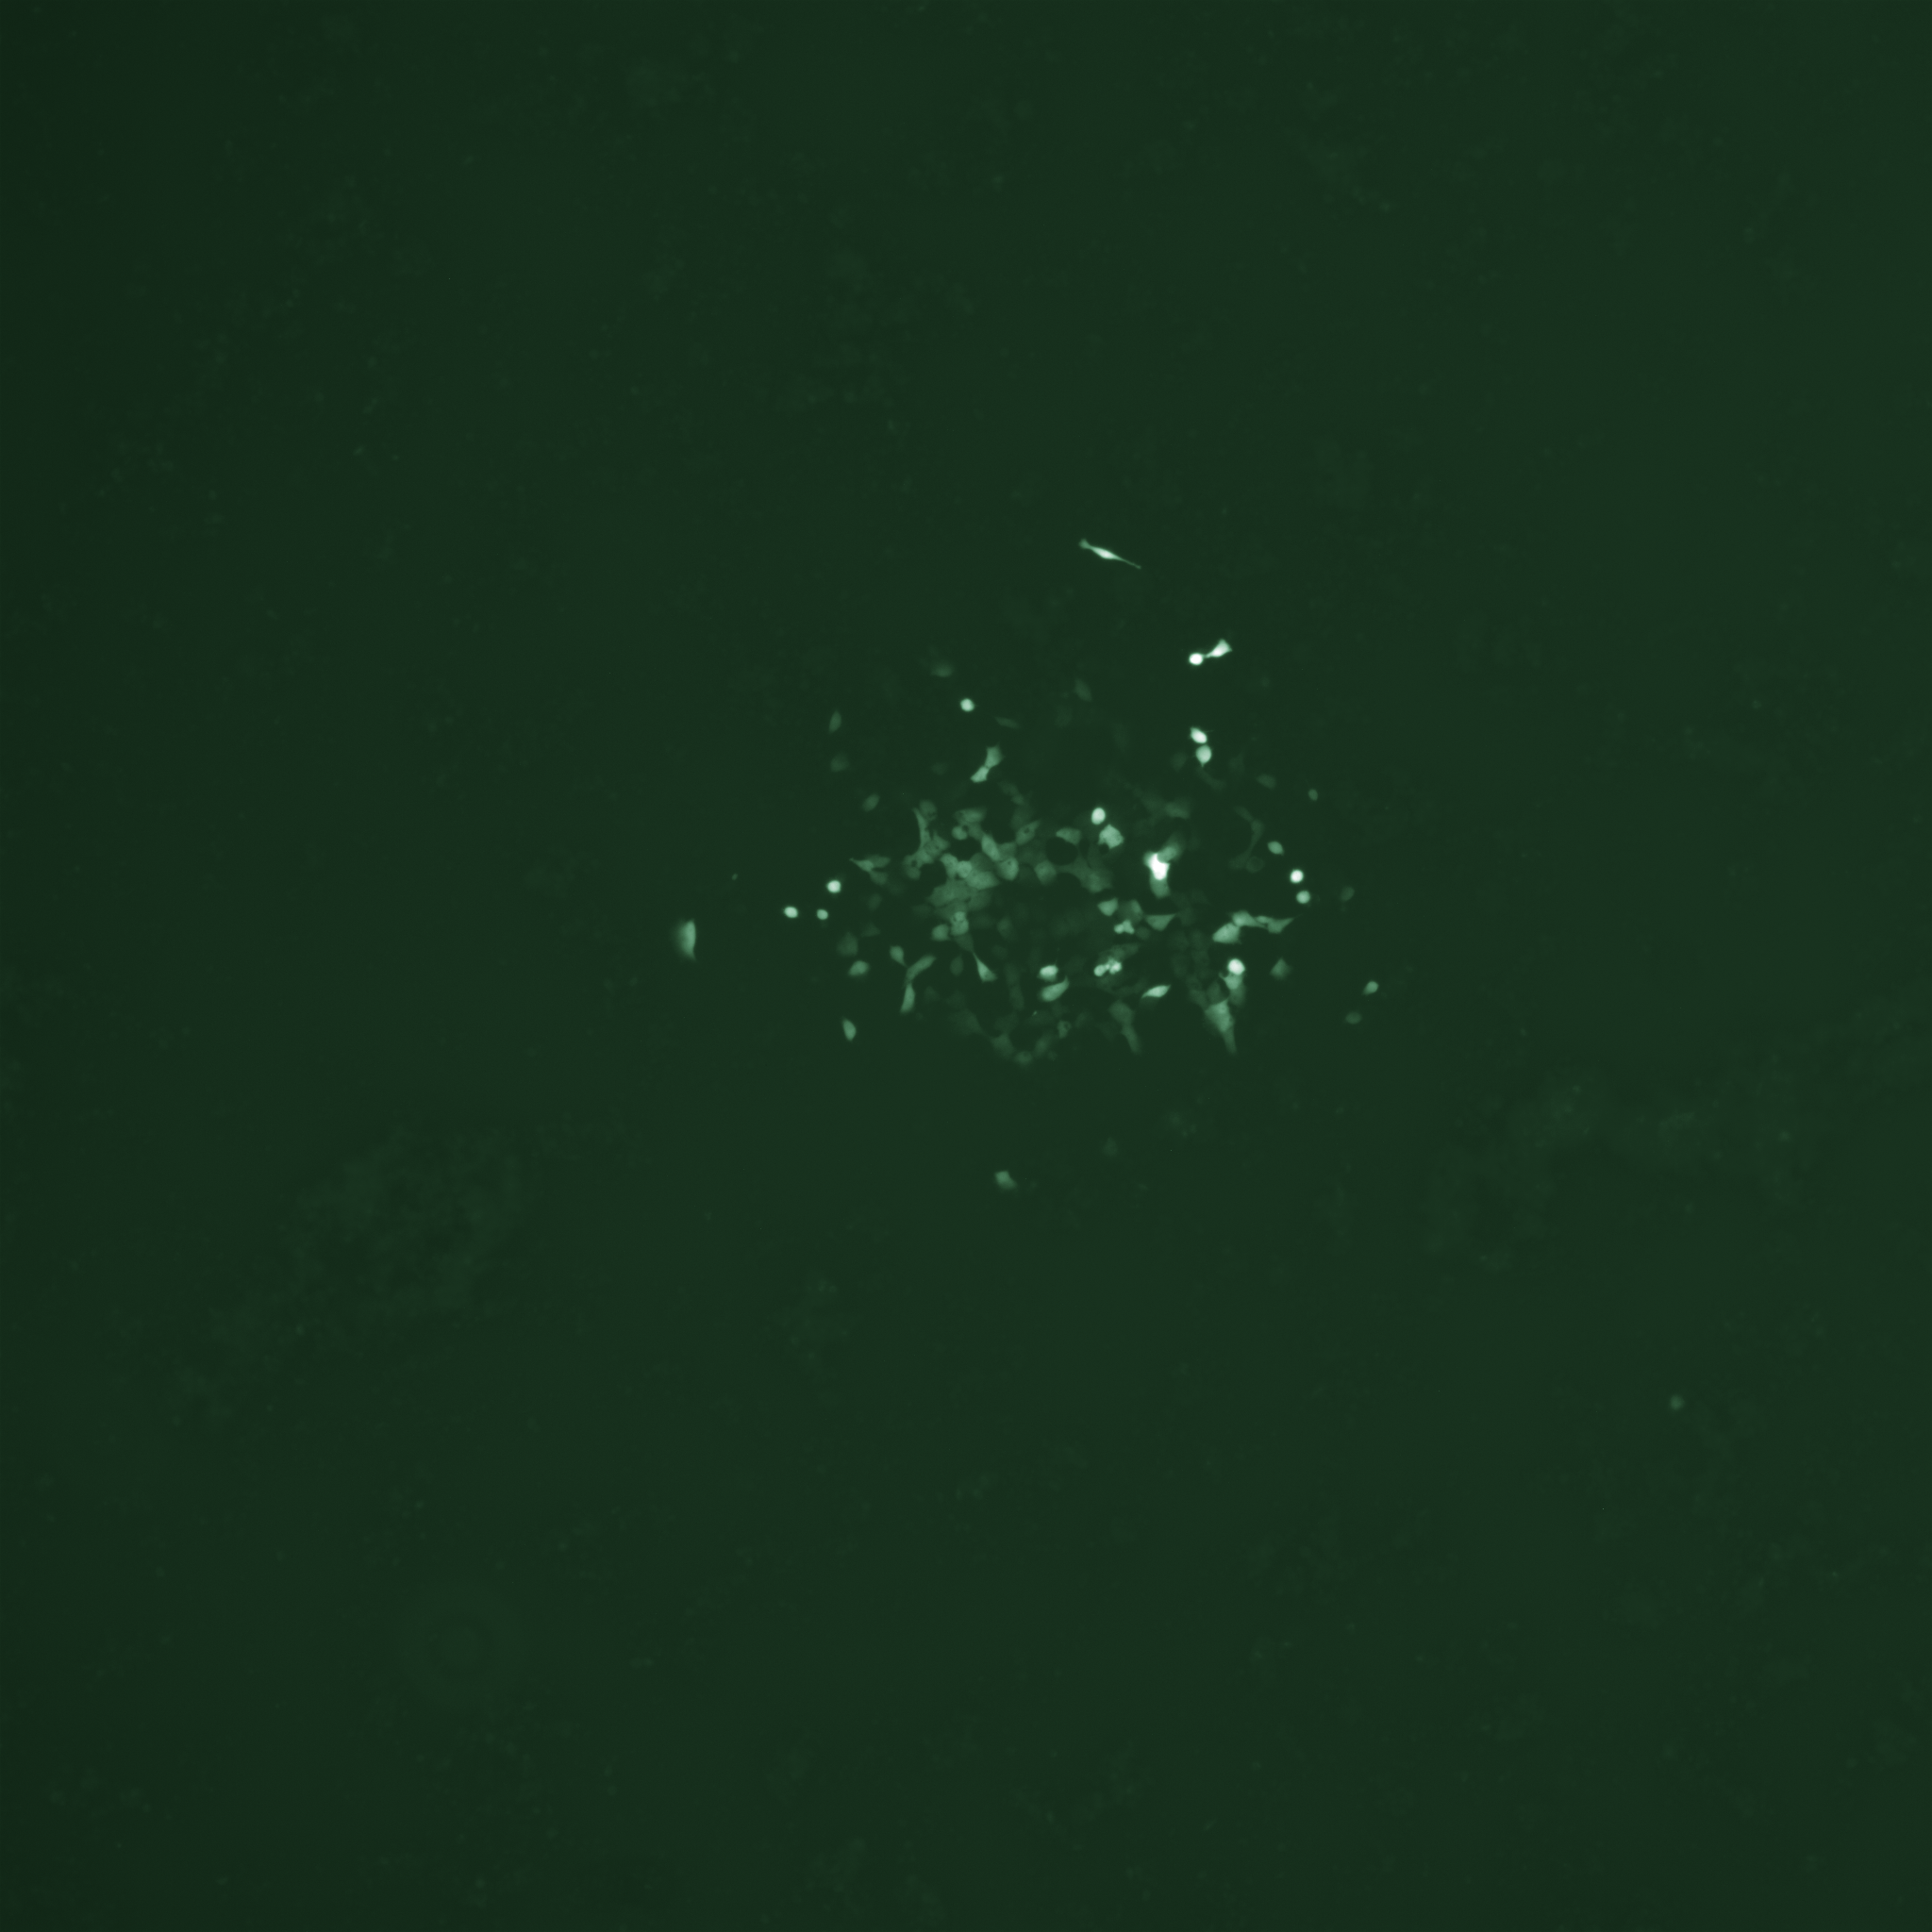
\includegraphics[width=0.25\linewidth]{Photos/74_GFP.png}\\
          e)
             \includegraphics[width=0.25\linewidth]{Photos/Mock_phase.png}
          f)
             \includegraphics[width=0.25\linewidth]{Photos/Mock_GFP.png}
      		\caption{A figure caption.}
    	\end{figure}
    	\end{column}
        
  		\begin{column}{0.49\linewidth}
    	Some sample text to see the size of a sub-column in the Results section.
    	\end{column}
  	\end{columns}
  \end{block}

\end{column}

\separatorcolumn
\setlength{\colwidth}{0.25\paperwidth}
\begin{column}{\colwidth}

  \begin{alertblock}{Future Directions}

    Nullam non est elit. In eu ornare justo. Maecenas porttitor sodales lacus,
    ut cursus augue sodales ac.

    $$
    \int_{-\infty}^{\infty} e^{-x^2}\,dx = \sqrt{\pi}
    $$

    Interdum et malesuada fames $\{1, 4, 9, \ldots\}$ ac ante ipsum primis in
    faucibus. Cras eleifend dolor eu nulla suscipit suscipit. Sed lobortis non
    felis id vulputate.

    \heading{A heading inside a block}

    Praesent consectetur mi $x^2 + y^2$ metus, nec vestibulum justo viverra
    nec. Proin eget nulla pretium, egestas magna aliquam, mollis neque. Vivamus
    dictum $\mathbf{u}^\intercal\mathbf{v}$ sagittis odio, vel porta erat
    congue sed. Maecenas ut dolor quis arcu auctor porttitor.

    \heading{Another heading inside a block}

    Sed augue erat, scelerisque a purus ultricies, placerat porttitor neque.
    Donec $P(y \mid x)$ fermentum consectetur $\nabla_x P(y \mid x)$ sapien
    sagittis egestas. Duis eget leo euismod nunc viverra imperdiet nec id
    justo.

  \end{alertblock}


  \begin{block}{References}

    \nocite{*}
    \footnotesize{\bibliographystyle{plain}\bibliography{SURFReferences}}

  \end{block}

\end{column}

\separatorcolumn
\end{columns}
\end{frame}

\end{document}
